Pose detection is done with OpenPose\footnote{\url{https://github.com/CMU-Perceptual-Computing-Lab/openpose}}.
OpenPose is a real-time multi-person keypoint detection library for body, face, and hands.
It's used for example in the restaurant challenge to detect waving persons.
In the finals we used it to detect when an operator points to objects in the living room.
For that we ray-traced the vector of the arm in our world model and extracted the first object that the ray intersects.
This enables the robot to understand commands like: ``Give me \emph{that} object''.
See figure \ref{fig:pose_detection} for an example of the output of the algorithm.

\begin{figure}[H]
	\centering
	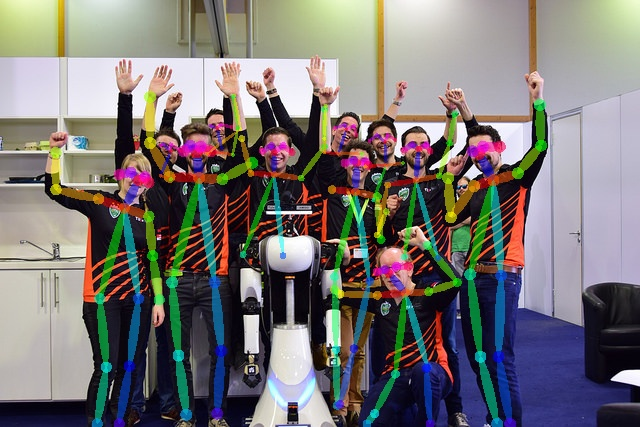
\includegraphics[width=0.66\linewidth]{openpose}
	\caption{Pose detection}
	\label{fig:pose_detection}
\end{figure}
